The burgeoning interest in Retrieval Augmented Generation (RAG) has led to a significant surge in the development of advanced Information Retrieval (IR) systems. Large Language Models (LLMs) in turn can now handle large contexts~\cite{chen2023extending,liu2024world}, though they suffer from a ``lost in the middle'' problem ~\cite{liu-etal-2024-lost,bai2024longbench,bai2024longbench2, Li2024LongcontextLS}. Therefore, retrieving precise information~\cite{Pipitone2024LegalBenchRAGAB} is extremely important to curb hallucinations~\cite{Laban2024SummaryOA} and generate accurate responses. Current retrievers address this by creating length based chunks~\cite{Setty2024ImprovingRF} and throwing away rich and informative semantic global structure in the corpus. This leads to a sub-optimal retrieval quality -- length-based chunks compete with each other due to a lack of semantic coherence and boundaries.

In this work, we address this key limitation by augmenting the retriever with a structured global view of the corpus. Global structured view over a long context helps knowledge ingestion~\cite{liu2024structureaware}. Further, LLMs are capable of storing the entire corpus in its model parameters to directly generate a document identifier for a user query~\cite{Tay2022TransformerMA}. We posit that by empowering an LLM with a global structure of the search corpus, it can store and retrieve information more accurately from its model parameters. Such a global structure already exists for a Wikipedia~\cite{wikipedia-sample-layout} page, textbooks, and enterprise help and product feature webpages~\cite{SAP-product-documentation} and technical reports~\cite{SEC-10k-structure}.

% We posit that an LLM which has successfully been shown to ingest the entire corpus within its model parameters~\cite{Tay2022TransformerMA} can further benefit by being cognizant of the global structure of the corpus. This could help LLM efficiently organize the information 

% In fact, it has been already shown that having a global structured view over a long context helps in knowledge intensive tasks such as knowledge ingestion . We bring the same intuition into the retrieval paradigm by using Table of Contents ({\toc}) as a form of hierarchical global structure over a long search context such as a voluminous book. As shown in Figure~\ref{fig:intro_example}, {\toc} lays out the structure of the book into different sections and subsections and so on with representative section titles highlighting what is expected in those sections. This acts as a useful prior to guide information search. {\toc}\ is quite common and readily available in academic settings such as Wikipedia~\cite{wikipedia-sample-layout} pages, educational books like we have used in this work, as well as enterprise settings such as product feature descriptions~\cite{SAP-product-documentation} or typical technical reports~\cite{SEC-10k-structure}

% Moreover, using {\toc} to represent global context has two key advantages: (1) {\toc}\ is quite common and readily available in academic settings such as wikipedia ~\cite{wikipedia-sample-layout} pages, educational books like we have used in this work, as well as enterprise settings such as product feature descriptions~\cite{SAP-product-documentation} or typical technical reports~\cite{SEC-10k-structure} and (2) existence of {\toc}\ is not a hard constraint anyway. As shown by previous works ~\cite{liu2024enhancing}, it is always possible to curate a ({\toc}) style semantic structure with desired level of granularity by summarizing different sections within the book. 

\begin{figure*}[!htb]
\begin{center}
    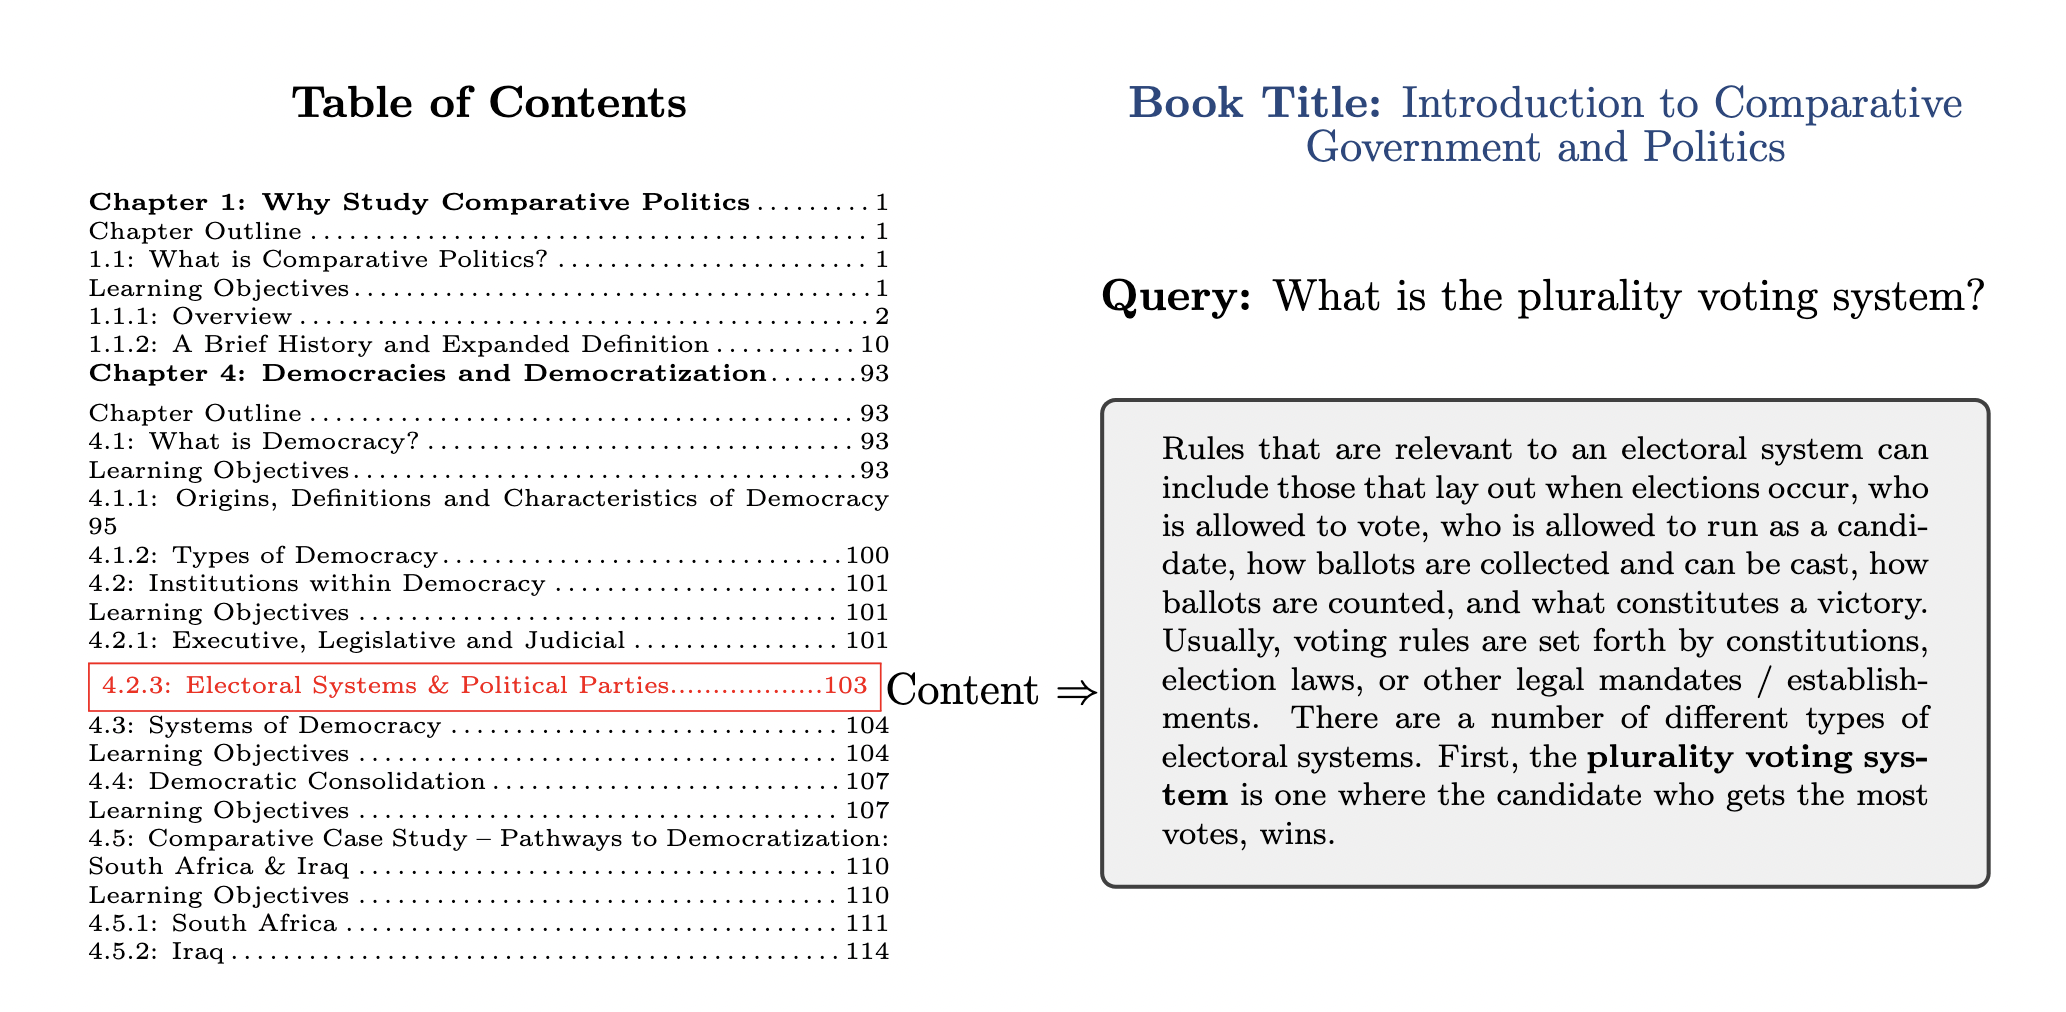
\includegraphics[width=\linewidth]{images/f1_latex}
    \caption{A human can answer ``What is the plurality voting system?'' by looking at the table of contents and picking Section 4.2.3 without even reading the book \href{https://open.umn.edu/opentextbooks/textbooks/1435}{Introduction to Comparative Government and Politics}.}
    % \caption{Can an IR system select the best leaf node which can answer a user query?}
    \label{fig:intro_example}
\end{center}
\end{figure*}

Figure~\ref{fig:intro_example} demonstrates that for a question such as ``What is the plurality voting system?'', it is  natural for a human to consult the {\toc} and first narrow down that it could be answered by the Chapter ``Democracies and Democratization''. Further subsections reveal that perhaps the Section ``Institutions within Democracy'' and the subsection ``Electoral Systems \& Political Parties'' could contain the answer. Content for this subsection indeed contains the definition for the plural voting system. Text content associated with {\toc} entries is semantically coherent organized around a topic as captured by the title of the {\toc} entry. Further, a {\toc} entry has a  clear semantic boundary with other {\toc} entries. {\toc} as a unit of retrieval is a novel yet intuitive way of organizing long context for retrieval.

% and move to the subsection titled \textit{} (Chapter  and Section ) to find relevant information needed to answer the question.

% Given the structure and organization of a long document $D$ in the form of table of contents ${\toc}_{D}$, the retrieval task is to retrieve the correct subsection $t_{l} \in {\toc}_{D}$ which contains content to answer the user query $q$.  Also, using ({\toc}) for retrieval naturally mimics a human like search behavior. Figure~\ref{fig:intro_example} demonstrates that a question such as \textit{``What is the plurality voting system?''}(Fig~\ref{fig:intro_example}), it is very natural for humans to consult the {\toc} and move to the subsection titled \textit{Electoral Systems \& Political Parties} (Chapter ``Democracies and Democratization'' and Section ``Institutions within Democracy'') to find relevant information needed to answer the question.
In this work, we present {\sys} (\textbf{ST}ructure \textbf{A}ware \textbf{I}nformation \textbf{R}etriever) for {\toc} based retrieval, inspired by how a human searches for information using {\toc}, and the fact that LLMs can store the entire corpus in the model's parameters. Our careful and thorough ablation studies reveal that empowering an LLM with {\toc} helps in two critical dimensions - curbing hallucinations and generalizing for content with a low number of training examples. {\sys} achieves a high Recall@1 score of 82.6, which is is ($+7.4\%$) better than its closest baseline Differentiable Search Index (DSI)~\cite{Tay2022TransformerMA}. DSI needs to discover the book structure (indirectly) through the completion part of training examples, while {\sys}\ can use exploit the structure provided as part of the input to accurately store and retrieve information from its model's parameters.

% We observe that if out-of-the-box LLMs use {\toc} for predicting right subsection identifier in zero shot setup, it's Recall@1 performance remains sub-optimal at only 13.8. But if the LLM is also tuned on the text content of the book along with {\toc} as an additional input, it sees a significant jump in Recall@1 with an average of 82.6. Our ablation study suggests that using {\toc} as input is vital for the success of {\sys}, as the core structure of the book captured in {\toc} helps {\sys} navigate the book's content during LLM fine-tuning. This helps {\sys} get good gains ($+7.4\%$) over its closest baseline Differential Search Index (DSI)~\cite{Tay2022TransformerMA}. We observe that DSI, when fine-tuned with the same book content but without using the {\toc}\ as input, performs poorly compared to {\sys}. This is because DSI needs to discover the book structure through the training examples, while {\sys}\ can use the structure already provided by the {\toc} as part of the input.

We develop and release a new multi-domain benchmark {\ben}, made up of $18$ books of varying sizes across $6$ domains, parsed and cleaned to extract their {\toc} mapped to the text of the pertinent sections. We also release a set of train, dev and test queries for each book as part of the benchmark, with gold {\toc} entries labeled for each query serving as the retrieval output. We believe this will be a first step towards promoting further research on {\toc} based retrieval, with {\ben} serving as a standard evaluation benchmark. We train and evaluate {\sys} using {\ben} and compare it with strong baseline retrievers like BM25 and a fully fine-tuned Sequence-to-Sequence model, such as DSI~\cite{Tay2022TransformerMA}, which does not utilize {\toc}. Our experimental results show that {\sys} significantly benefits from incorporating {\toc} in its training and easily outperforms the traditional DSI. Our main contributions are as follows:
\begin{itemize}
\item We propose a novel direction leveraging the Table of Contents ({\toc}) of a lengthy corpus, like a book, as a valuable element for efficiently indexing corpus knowledge and utilizing {\toc} entries as effective retrieval units.
\item We build and release a multi-domain and diverse benchmark {\ben}, consisting of $18$ books from $6$ diverse domains for the task of {\toc} retrieval
\item We develop an LLM based {\sys} and evaluate it on {\ben} and compare it with strong competitive baselines
\end{itemize}